%%%%%%%%%%%%%%%%%%%%%%%%%%%%%%%%%%%%%%%%%
% SLIIT Metropolitan Campus
% Enterprise Software Analysis & Design
% SE5060: Exercise 9
% Version 1.0 (2020-09-08)
%
% Authors:
% Pradeep (sanjayangp@gmail.com)

%
% License:
% CC BY-NC-SA 3.0 (http://creativecommons.org/licenses/by-nc-sa/3.0/)
% 
%%%%%%%%%%%%%%%%%%%%%%%%%%%%%%%%%%%%%%%%%

%----------------------------------------------------------------------------------------
%	PACKAGES AND OTHER DOCUMENT CONFIGURATIONS
%----------------------------------------------------------------------------------------

\documentclass[12pt]{scrartcl} % Font size

\usepackage{amsmath, amsfonts, amsthm} % Math packages

\usepackage{listings} % Code listings, with syntax highlighting

\usepackage[english]{babel} % English language hyphenation

\usepackage{graphicx} % Required for inserting images
\graphicspath{{Figures/}{./}} % Specifies where to look for included images (trailing slash required)

\usepackage{booktabs} % Required for better horizontal rules in tables
\usepackage[shortlabels]{enumitem}
\usepackage{float}


\numberwithin{equation}{section} % Number equations within sections (i.e. 1.1, 1.2, 2.1, 2.2 instead of 1, 2, 3, 4)
\numberwithin{figure}{section} % Number figures within sections (i.e. 1.1, 1.2, 2.1, 2.2 instead of 1, 2, 3, 4)
\numberwithin{table}{section} % Number tables within sections (i.e. 1.1, 1.2, 2.1, 2.2 instead of 1, 2, 3, 4)

\setlength\parindent{0pt} % Removes all indentation from paragraphs

\usepackage{enumitem} % Required for list customisation
\setlist{noitemsep} % No spacing between list items

%----------------------------------------------------------------------------------------
%	DOCUMENT MARGINS
%----------------------------------------------------------------------------------------

\usepackage{geometry} % Required for adjusting page dimensions and margins

\geometry{
	paper=a4paper, % Paper size, change to letterpaper for US letter size
	top=2.5cm, % Top margin
	bottom=3cm, % Bottom margin
	left=3cm, % Left margin
	right=3cm, % Right margin
	headheight=0.75cm, % Header height
	footskip=1.5cm, % Space from the bottom margin to the baseline of the footer
	headsep=0.75cm, % Space from the top margin to the baseline of the header
	%showframe, % Uncomment to show how the type block is set on the page
}

%----------------------------------------------------------------------------------------
%	FONTS
%----------------------------------------------------------------------------------------

\usepackage[utf8]{inputenc} % Required for inputting international characters
\usepackage[T1]{fontenc} % Use 8-bit encoding

\usepackage{times} % Use the Adobe Utopia font for the document

%----------------------------------------------------------------------------------------
%	SECTION TITLES
%----------------------------------------------------------------------------------------

\usepackage{sectsty} % Allows customising section commands

\sectionfont{\vspace{6pt}\centering\normalfont\scshape} % \section{} styling
\subsectionfont{\normalfont\bfseries} % \subsection{} styling
\subsubsectionfont{\normalfont\itshape} % \subsubsection{} styling
\paragraphfont{\normalfont\scshape} % \paragraph{} styling

%----------------------------------------------------------------------------------------
%	HEADERS AND FOOTERS
%----------------------------------------------------------------------------------------

\usepackage{scrlayer-scrpage} % Required for customising headers and footers

\ohead*{} % Right header
\ihead*{} % Left header
\chead*{} % Centre header

\ofoot*{} % Right footer
\ifoot*{} % Left footer
\cfoot*{\pagemark} % Centre footer
 % Include the file specifying the document structure and custom commands

%----------------------------------------------------------------------------------------
%	TITLE SECTION
%----------------------------------------------------------------------------------------

\title{	
	\normalfont\normalsize
	\textsc{Master of Science in Information Technology Specializing in Enterprise Applications Development}\\
	\textsc{SLIIT Metropolitan Campus}\\
	\textsc{BOC Merchant Tower, No \#28, St Michae\rq{}s Road,}\\
	\textsc{Colombo 03, Sri Lanka}\\
	\vspace{25pt} % Whitespace
	\rule{\linewidth}{0.5pt}\\ % Thin top horizontal rule
	\vspace{20pt} % Whitespace
	{\huge Enterprise Software Analysis \& Design}\\
	\textsc{SE5060: Exercise 9}\\
	\vspace{12pt} % Whitespace
	\rule{\linewidth}{2pt}\\ % Thick bottom horizontal rule
	\vspace{12pt} % Whitespace
}

\author{\LARGE N. G. Pradeep Sanjaya\\
	\small{MS20921576}
} % Your name

\date{\normalsize\today} % Today's date (\today) or a custom date

\begin{document}

\maketitle % Print the title

\newpage
\section*{Answer}
Github - https://github.com/pradeep-sanjaya/ead-esad-exercise9

\subsection*{Classes}


\textbf{AdapterTest.java}
\lstset{language=Java}
\begin{lstlisting}[frame=single]
package com.sliit;

import com.sliit.impl.PersonImpl;
import com.sliit.impl.RemotePersonImpl;

public class AdapterTest {
  public static void main(String[] args) {
    Person person = new PersonImpl();
    RemotePerson remotePerson = new RemotePersonImpl();

    System.out.println("Person says");
    System.out.println(person.generateFullName());
    System.out.println(person.generateFullAddress());

    System.out.println("\nRemote person says");
    System.out.println(remotePerson.getFirstName());
    System.out.println(remotePerson.getLastName());
    System.out.println(remotePerson.getAddressLine1());
    System.out.println(remotePerson.getAddressLine2());

    System.out.println("\nPerson adapter says");
    PersonAdapter personAdapter = new PersonAdapter(remotePerson);
    System.out.println(personAdapter.generateFullName());
    System.out.println(personAdapter.generateFullAddress());
  }
}
\end{lstlisting}


\textbf{Person.java}
\lstset{language=Java}
\begin{lstlisting}[frame=single]
package com.sliit;

public interface Person {
  String generateFullName();
  String generateFullAddress();
}
\end{lstlisting}

\textbf{PersonImpl.java}
\lstset{language=Java}
\begin{lstlisting}[frame=single]
package com.sliit.impl;

import com.sliit.Person;

public class PersonImpl implements Person {

  private static String FULL_NAME    = "Pradeep Sanjaya";
  private static String FULL_ADDRESS = "Pothuarawa Road, Malabe";

  @Override
  public String generateFullName() {
    return FULL_NAME;
  }

  @Override
  public String generateFullAddress() {
    return FULL_ADDRESS;
  }
}
\end{lstlisting}

\textbf{RemotePerson.java}
\lstset{language=Java}
\begin{lstlisting}[frame=single]
package com.sliit;

public interface RemotePerson {
  String getFirstName();
  String getLastName();
  String getAddressLine1();
  String getAddressLine2();
}
\end{lstlisting}

\textbf{RemotePersonImpl.java}
\lstset{language=Java}
\begin{lstlisting}[frame=single]
package com.sliit.impl;

import com.sliit.RemotePerson;

public class RemotePersonImpl implements RemotePerson {

  private static String FIRST_NAME = "Pradeep";
  private static String LAST_NAME  = "Sanjaya";
  private static String ADDRESS1   = "Pothuarawa Road";
  private static String ADDRESS2   = "Malabe";

  @Override
  public String getFirstName() {
    return FIRST_NAME;
  }

  @Override
  public String getLastName() {
    return LAST_NAME;
  }

  @Override
  public String getAddressLine1() {
    return ADDRESS1;
  }

  @Override
  public String getAddressLine2() {
    return ADDRESS2;
  }
}
\end{lstlisting}


\textbf{PersonAdapter.java}
\lstset{language=Java}
\begin{lstlisting}[frame=single]
package com.sliit;

public class PersonAdapter implements Person {

  private static String SEPERATOR = " ";

  RemotePerson remotePerson;

  public PersonAdapter(RemotePerson remotePerson) {
    this.remotePerson = remotePerson;
  }

  @Override
  public String generateFullName() {
    StringBuilder stringBuilder = new StringBuilder();
    stringBuilder.append(remotePerson.getFirstName());
    stringBuilder.append(SEPERATOR);
    stringBuilder.append(remotePerson.getLastName());
    return stringBuilder.toString();
  }

  @Override
  public String generateFullAddress() {
    StringBuilder stringBuilder = new StringBuilder();
    stringBuilder.append(remotePerson.getAddressLine1());
    stringBuilder.append(SEPERATOR);
    stringBuilder.append(remotePerson.getAddressLine2());
    return stringBuilder.toString();
  }
}
\end{lstlisting}


\subsection*{Screenshots}
\begin{center}
	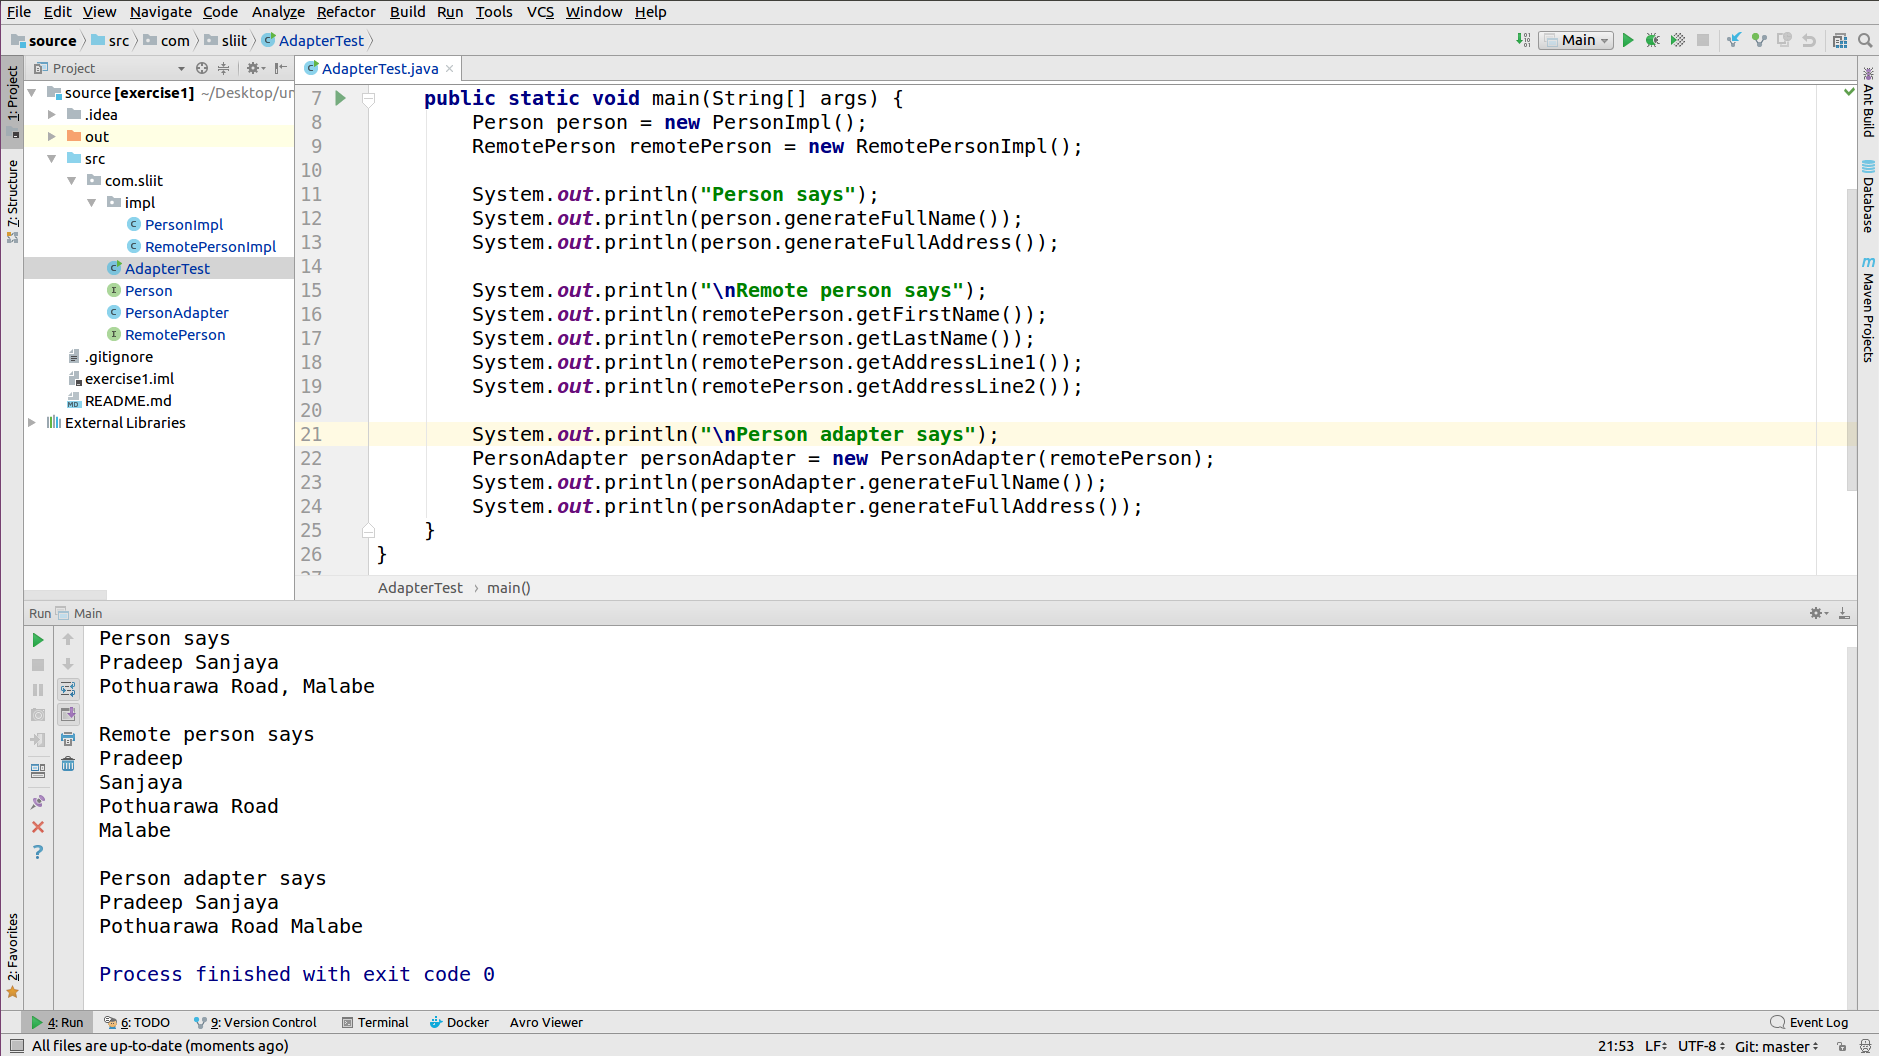
\includegraphics[width=1.0\columnwidth]{./figures/01.png}
	\captionof{figure}{Solution}\label{Solution}%
\end{center}


\pagebreak
\newpage
\begin{thebibliography}{00}
	\raggedright
	\bibitem{b1} Samarathunge, U. (2020) Lecture - 03 GOF Design Patterns Part I
    \bibitem{b2} Samarathunge, U. (2020) Lecture - 03 GOF Design Patterns Part II-v2
    \bibitem{b3} Samarathunge, U. (2020) Lecture - 03 GOF Design Patterns Part II With Answers
    \bibitem{b4} Samarathunge, U. (2020) Lecture - 03 GOF Design Patterns Part III
\end{thebibliography}


\end{document}
